
\documentclass[12pt]{article}
\usepackage{times}
\usepackage{titling}
\usepackage{enumitem}
\usepackage{graphicx}
\usepackage{float}
\usepackage{longtable}

\setlength{\droptitle}{-10em} 

\title{System Requirements Specifications\\
	\large Agar.io for SE 3XA3}
\author{Yash Gopal, Vicky Bilbily, and Jemar Jones.}
\date{October 10, 2015}

\begin{document}


\maketitle
\tableofcontents
\newpage

\section{Project Drivers}
\subsection{Purpose of the Project}
\textbf{The User Business or Background of the Project Effort}
The purpose of Agar.io is to reinvent the way simple multiplayer games work and provide inspiration to the open source game development community. Most multiplayer games nowadays whether they are web-based, desktop, console or mobile, require signups. This is meant to be extremely easy to jump into while still providing a competitive and challenging environment to keep the user engaged and addicted.

The game itself revolves around players starting off as small blobs who can then move around and consume other player blobs to keep increasing in size. Your goal is to be the biggest fish in the pond. However, there’s a catch. The bigger you are, the slower you get and there are plenty of other players on the playing field. The player has to be smart and quick witted to climb the score board.
\subsection{The Client, the Customer and other Stakeholders}
The purpose of Agar.io is to reinvent the way simple multiplayer games work and provide inspiration to the open source game development community. Most multiplayer games nowadays whether they are web-based, desktop, console or mobile, require signups. This is meant to be extremely easy to jump into while still providing a competitive and challenging environment to keep the user engaged and addicted.

The game itself revolves around players starting off as small blobs who can then move around and consume other player blobs to keep increasing in size. Your goal is to be the biggest fish in the pond. However, there’s a catch. The bigger you are, the slower you get and there are plenty of other players on the playing field. The player has to be smart and quick witted to climb the score board.
\subsection{Users of the Product}
\textbf{Hands-On Users}

The initial users of the product will be limited to our team and the students enrolled in the 3XA3 course.

Once the project goes live on a public domain, the users will be anyone with access to the website from a Windows, Mac OSX or mobile OS platform like iOS or Android.

All users are assumed to have some experience with games and how they work.\\
\textbf{Priorities Assigned to Users}\\

\textbf{Key Users:} General Public (Windows, Mac OSX, iOS & Android)

\textbf{Secondary Users:} Professor, Developers and Testers\\\\
\textbf{User Participation}
\begin{enumerate}
\item Users playing the game are prompted to use an anonymous name that they can create. No credentials are needed or stored.
\item No user data is stored. Every session requires a new name to be created by the user.
\end{enumerate}
Maintenance Users and Service Technicians

These are the developers. (Our team)
\section{Project Constraints}
\subsection{Mandated Constraints}
\textbf{Solution Constraints}

The most important mandated constraint is the server. We will be hosting the game on our own server which means the game can only support a certain number of concurrent players before reaching a performance threshold. This also means latency will differ greatly based on where the game is accessed from.\\
\textbf{Implementation Environment}

The coding languages used will be web technologies such as HTML5, CSS3 and Javascript.
Frameworks such as Socket.io, jQuery, Fabric.js, Paper.js, Create.js and Bootstrap will also be utilized.
Node.js is a javascript runtime environment that will be used along with Socket.io to create the server and host the game.
The development will utilize code editors such as Brackets or Sublime Text. We will also be using Bash or Windows PowerShell to commit & push and run appropriate documentation tools.\\
\textbf{Partner or Collaborative Applications}

not applicable\\
\textbf{Off-the-shelf Software}

not applicable\\
\textbf{Anticipated Workplace Environment}

This game will be mostly used at home and on the move.\\
\textbf{Schedule Constraints}

The deadline for the project is around mid-December, which gives our team around 3 months of development time.

Final Demo: Week of November 30th, 2015 
Final Documentation: December 8th, 2015\\
\textbf{Budget Constraints}

not applicable
\subsection{Naming Conventions & Terminology}
\begin{itemize}
\item{Port: The Node.js server will run on a certain network location also known as the port.}
\item{Ping: The latency between the client playing the game and the server.}
\item{Web socket: Allows a persistent connection between the client and the server which means both parties can start sending data at any time without requiring an HTTP connection or long polling.}
\end{itemize}
\subsection{Relevant Facts & Assumptions}

Facts

People love games. A simple, fast-paced and challenging game that users can play anywhere, anytime with no time commitment is most likely to be highly successful.

Assumptions

The game will only run well on the future-friendly browsers such as Google Chrome, Safari and Mozilla Firefox. Thus we are assuming the game will mostly be played on these browsers whether on desktop or mobile.
\section{Functional Requirements}
\subsection{The Scope of the Work}
	\textbf{a) The Current Situation}

	A very basic Node.js server application exists and can be deployed from any
	modern Windows, OS X, or Linux environment.
	
	\textbf{b) The Context of the Work}
	\begin{figure}[H]
	\centering
	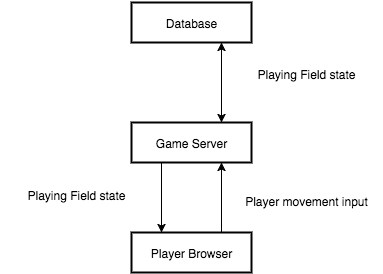
\includegraphics[width=90mm]{contextsrs.png}
	\caption{Context diagram \label{overflow}}
	\end{figure}
	
	\textbf{c) Work Partitioning}

    \begin{longtable}{ | l | p{3cm}  | p{3cm} |}
    \hline
    Event Name & input/output & Summary \\ \hline
    1. Player Enters game & Player ID (IN) Player Position (OUT) Player Mass (OUT) Field state (OUT) & Player chooses name and is placed in the live game. \\ \hline
    2. Player changes position/direction & Player Position (IN) Player Mass (OUT) Field state (OUT) & Player indicates the position/direction they will move in, this is synced with the current Field State. \\ \hline
    3. Player eats food/another player & Player Position (IN) Player Mass (OUT) Field state (OUT) & Players new position overlaps with smaller food/player, the food/player dissapears and its mass is added to the Player\\ \hline
    4. Player is eaten & Player Final Score & Player is eaten and is givin info on there final score.\\ \hline
    \caption{Work Partitioning}
    \end{longtable}
\subsection{The Scope of the Product}
\textbf{a) Product Boundary}

See Figure 1\\
\textbf{b) Product Use Case List}
\begin{figure}[H]
\centering
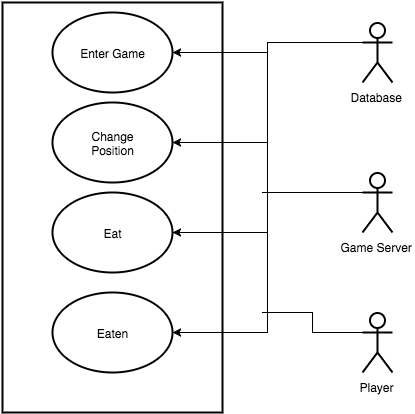
\includegraphics[width=90mm]{SRScase.png}
\caption{Case diagram \label{overflow}}
\end{figure}

\textbf{c) Individual Product Use Cases}\newline\\
1. Product Use Case Name: Enter Game\newline
Trigger: Player types name and presses play. \newline
Preconditions: A player is not already in the middle of a game. \newline
Interested Stakeholders: The player, the client, and the developers. \newline
Actors: Player, Game Server, Database \newline
Outcome: If the users name is not already taken, then they are now a player in the currently live game session.\newline\\
2. Product Use Case Name: Change Position\newline
Trigger: Player moves pointer in the direction of the new position.\newline
Preconditions: Player is currently playing the game, is still alive, and there is a position in the direction the player has placed their pointer. \newline
Interested Stakeholders: The player, the client, and the developers. \newline
Actors: Player, Game Server, Database \newline
Outcome: The player is moved to a position an increment of X away in the direction the pointer was placed (relative to their current position).\newline\\
3. Product Use Case Name: Eat\newline
Trigger: A players position completely overlaps the position of a smaller food/other player. \newline
Preconditions: Player is currently playing the game, and is still alive. \newline
Interested Stakeholders: The player, the client, and the developers. \newline
Actors: Player, Game Server, Database \newline
Outcome: The food or other player dissapears and/or dies. The player doing the "eating" has their mass increase by the mass of the food/other player at the time of "eating".\newline\\
4. Product Use Case Name: Eaten\newline
Trigger: A players position is completely overlapped by another larger player.\newline
Preconditions: Player is currently playing the game, and is still alive. \newline
Interested Stakeholders: The player, the client, and the developers. \newline
Actors: Player, Game Server, Database \newline
Outcome: The players screen goes black, they are told theyve died, and there final score/mass is displayed. Afer a brief moment they are allowed to enter the game again if they wish. \newline
\subsection{Functional and Data Requirements}

\textbf{a) Functional Requirements}
\medskip 

\fbox{
	\parbox{\textwidth}{
		\textbf{Requirement \#:} 1 \ \ 
		\textbf{Requirement Type:} 9 \ \ 
		\textbf{Event/Use case \#:} 1 \\
		\textbf{Description:} The game must be accessible online. \\
		\textbf{Rationale:} It is an online, multiplayer game. \\
		\textbf{Originator:} Vicky Bilbily \\
		\textbf{Fit Criterion:} The game is accessed via URL through a web browser that is connected to the internet. \\
		\textbf{Customer Satisfaction:} 5 \ \ 
		\textbf{Customer Dissatisfaction:} 5 \\
		\textbf{Priority:} High \ \ 
		\textbf{Conflicts:} None \\
		\textbf{Supporting Material:} None \\
		\textbf{History:} Created October 10, 2015
	}
}

\bigskip

\fbox{
	\parbox{\textwidth}{
		\textbf{Requirement \#:} 2 \ \ 
		\textbf{Requirement Type:} 9 \ \ 
		\textbf{Event/Use case \#:} 1 \\
		\textbf{Description:}  The user must be able to join the online game at any time.\\
		\textbf{Rationale:}  There is one instance of the game that is ongoing.\\
		\textbf{Originator:} Vicky Bilbily \\
		\textbf{Fit Criterion:}  The user successfully joins the game.\\
		\textbf{Customer Satisfaction:} 5 \ \ 
		\textbf{Customer Dissatisfaction:} 5 \\
		\textbf{Priority:} High\ \ 
		\textbf{Conflicts:} None \\
		\textbf{Supporting Material:} None \\
		\textbf{History:} Created October 10, 2015
	}
}

\bigskip

\fbox{
	\parbox{\textwidth}{
		\textbf{Requirement \#:}  3 \ \ 
		\textbf{Requirement Type:} 9 \ \ 
		\textbf{Event/Use case \#:} 1 \\
		\textbf{Description:} 	The user must be able to exit the game at any time. \\
		\textbf{Rationale:} The user will want to exit eventually. \\
		\textbf{Originator:} Vicky Bilbily \\
		\textbf{Fit Criterion:} User successfully exits game. \\
		\textbf{Customer Satisfaction:} 5 \ \ 
		\textbf{Customer Dissatisfaction:}  \\
		\textbf{Priority:} High \ \ 
		\textbf{Conflicts:} None \\
		\textbf{Supporting Material:} None \\
		\textbf{History:} Created October 10, 2015
	}
} \bigskip


\fbox{
	\parbox{\textwidth}{
		\textbf{Requirement \#:} 4 \ \ 
		\textbf{Requirement Type:} 9 \ \ 
		\textbf{Event/Use case \#:} 2 \\
		\textbf{Description:} All online players must exist simultaneously on the same game-field. \\
		\textbf{Rationale:} The game requires players to interact. \\
		\textbf{Originator:} Vicky Bilbily \\
		\textbf{Fit Criterion:} The game successfully keeps track of all online players. \\
		\textbf{Customer Satisfaction:} 5 \ \ 
		\textbf{Customer Dissatisfaction:} 5 \\
		\textbf{Priority:} High \ \ 
		\textbf{Conflicts:} None \\
		\textbf{Supporting Material:} None \\
		\textbf{History:} Created October 10, 2015
	}
} \bigskip


\fbox{
	\parbox{\textwidth}{
		\textbf{Requirement \#:} 5 \ \ 
		\textbf{Requirement Type:} 9 \ \ 
		\textbf{Event/Use case \#:} 2 \\
		\textbf{Description:} The user must be able to move their character around the game-field. \\
		\textbf{Rationale:} It is essential to the objective of the game that characters can move. \\
		\textbf{Originator:} Vicky Bilbily \\
		\textbf{Fit Criterion:} User-input is output into viewable motion by the game. \\
		\textbf{Customer Satisfaction:} 5 \ \ 
		\textbf{Customer Dissatisfaction:} 5 \\
		\textbf{Priority:} High \ \ 
		\textbf{Conflicts:} None \\
		\textbf{Supporting Material:} None \\
		\textbf{History:} Created October 10, 2015
	}
} \bigskip


\fbox{
	\parbox{\textwidth}{
		\textbf{Requirement \#:} 6 \ \ 
		\textbf{Requirement Type:} 9 \ \ 
		\textbf{Event/Use case \#:} 2 \\
		\textbf{Description:} The user's character must grow in weight but decrease in speed when they collide with objects or players smaller than them, essentially consuming them. \\
		\textbf{Rationale:} This is the core game-mechanic. \\
		\textbf{Originator:} Vicky Bilbily \\
		\textbf{Fit Criterion:} A character consumes another character and the game registers their increase in weight. \\
		\textbf{Customer Satisfaction:} 5 \ \ 
		\textbf{Customer Dissatisfaction:} 5 \\
		\textbf{Priority:} High \ \ 
		\textbf{Conflicts:} None \\
		\textbf{Supporting Material:} None \\
		\textbf{History:} Created October 10, 2015
	}
} \bigskip


\fbox{
	\parbox{\textwidth}{
		\textbf{Requirement \#:} 7 \ \ 
		\textbf{Requirement Type:} 9 \ \ 
		\textbf{Event/Use case \#:} 4 \\
		\textbf{Description:} The user's game must end when they are consumed. \\
		\textbf{Rationale:} This is how the consumption mechanic works. \\
		\textbf{Originator:} Vicky Bilbily \\
		\textbf{Fit Criterion:} A larger character collides with the user's character, and they are returned to the start screen. \\
		\textbf{Customer Satisfaction:} 5 \ \ 
		\textbf{Customer Dissatisfaction:} 5 \\
		\textbf{Priority:} High \ \ 
		\textbf{Conflicts:} None \\
		\textbf{Supporting Material:} None \\
		\textbf{History:} Created October 10, 2015
	}
} \bigskip


\fbox{
	\parbox{\textwidth}{
		\textbf{Requirement \#:} 8 \ \ 
		\textbf{Requirement Type:} 9 \ \ 
		\textbf{Event/Use case \#:} 3/4 \\
		\textbf{Description:} The game must keep track of character weights and collisions. \\
		\textbf{Rationale:} This data is necessary in order to keep the game going. \\
		\textbf{Originator:} Vicky Bilbily \\
		\textbf{Fit Criterion:} A user's weight is consistent with the amount they have consumed. \\
		\textbf{Customer Satisfaction:} 5 \ \ 
		\textbf{Customer Dissatisfaction:} 5 \\
		\textbf{Priority:} High \ \ 
		\textbf{Conflicts:} None \\
		\textbf{Supporting Material:} None \\
		\textbf{History:} Created October 10, 2015
	}
} \bigskip


\fbox{
	\parbox{\textwidth}{
		\textbf{Requirement \#:} 9 \ \ 
		\textbf{Requirement Type:} 9 \ \ 
		\textbf{Event/Use case \#:} 1 \\
		\textbf{Description:} When the user starts the game, their character's weight is set to the default minimum. \\
		\textbf{Rationale:} Fairness and consistency. \\
		\textbf{Originator:} Vicky Bilbily \\
		\textbf{Fit Criterion:} The weight of a character when entering a game is the same as the weight of any other character when they entered the game. \\
		\textbf{Customer Satisfaction:} 4 \ \ 
		\textbf{Customer Dissatisfaction:} 4 \\
		\textbf{Priority:} High \ \ 
		\textbf{Conflicts:} None \\
		\textbf{Supporting Material:} None \\
		\textbf{History:} Created October 10, 2015
	}
} \bigskip

\fbox{
	\parbox{\textwidth}{
		\textbf{Requirement \#:} 10 \ \ 
		\textbf{Requirement Type:} 9 \ \ 
		\textbf{Event/Use case \#:} 2 \\
		\textbf{Description:} The game must periodically add new objects to the board where they have been consumed. \\
		\textbf{Rationale:} In order for the game to continue, there must always be a way for characters to grow in weight. \\
		\textbf{Originator:} Vicky Bilbily \\
		\textbf{Fit Criterion:} A character consumes an object, then it reappears after some amount of time. \\
		\textbf{Customer Satisfaction:} 4 \ \ 
		\textbf{Customer Dissatisfaction:} 5 \\
		\textbf{Priority:} High \ \ 
		\textbf{Conflicts:} None \\
		\textbf{Supporting Material:} None \\
		\textbf{History:} Created October 10, 2015
	}
} \bigskip

\textbf{b) Data Requirements \\}
	Not applicable to this project.

\section{Non-functional Requirements}

\textbf{a) Appearance Requirements}
\medskip 


\fbox{
	\parbox{\textwidth}{
		\textbf{Requirement \#:} 11 \ \ 
		\textbf{Requirement Type:} 10 \ \ 
		\textbf{Event/Use case \#:} 2 \\
		\textbf{Description:} The game must display characters as circles whose sizes correspond to their weights. \\
		\textbf{Rationale:} Allows users to distinguish the weights of characters easily. \\
		\textbf{Originator:} Vicky Bilbily \\
		\textbf{Fit Criterion:}  \\
		\textbf{Customer Satisfaction:} 5 \ \ 
		\textbf{Customer Dissatisfaction:} 5 \\
		\textbf{Priority:} \ \ 
		\textbf{Conflicts:} None \\
		\textbf{Supporting Material:} None \\
		\textbf{History:} Created October 10, 2015
	}
} \bigskip


\fbox{
	\parbox{\textwidth}{
		\textbf{Requirement \#:} 12 \ \ 
		\textbf{Requirement Type:} 10 \ \ 
		\textbf{Event/Use case \#:} 1 \\
		\textbf{Description:} The game must display characters in various colours. \\
		\textbf{Rationale:} Colours make it easier for users to distinguish between characters. \\
		\textbf{Originator:} Vicky Bilbily \\
		\textbf{Fit Criterion:}  \\
		\textbf{Customer Satisfaction:} 4 \ \ 
		\textbf{Customer Dissatisfaction:} 3 \\
		\textbf{Priority:} \ \ 
		\textbf{Conflicts:} None \\
		\textbf{Supporting Material:} None \\
		\textbf{History:} Created October 10, 2015
	}
} \bigskip


\fbox{
	\parbox{\textwidth}{
		\textbf{Requirement \#:} 13 \ \ 
		\textbf{Requirement Type:} 10 \ \ 
		\textbf{Event/Use case \#:} 1 \\
		\textbf{Description:} The game must display the user's chosen player-name over top of their character. \\
		\textbf{Rationale:} Names allow even further distinguishing between characters. \\
		\textbf{Originator:} Vicky Bilbily \\
		\textbf{Fit Criterion:}  \\
		\textbf{Customer Satisfaction:} 4 \ \ 
		\textbf{Customer Dissatisfaction:} 3 \\
		\textbf{Priority:} \ \ 
		\textbf{Conflicts:} None \\
		\textbf{Supporting Material:} None \\
		\textbf{History:} Created October 10, 2015
	}
} \bigskip 

\textbf{b) Style Requirements \\}
Not applicable to this project. \\
\medskip

11. Usability and Humanity Requirements \\
\textbf{a) Ease of Use Requirements}
\medskip


\fbox{
	\parbox{\textwidth}{
		\textbf{Requirement \#:} 14 \ \ 
		\textbf{Requirement Type:} 11 \ \ 
		\textbf{Event/Use case \#:} All \\
		\textbf{Description:} The game must be easy to use by the average internet-user. \\
		\textbf{Rationale:} The target audience is internet-users. \\
		\textbf{Originator:} Vicky Bilbily \\
		\textbf{Fit Criterion:} An internet-user of any age or background is able to start and play the game without assistance. \\
		\textbf{Customer Satisfaction:} 5 \ \ 
		\textbf{Customer Dissatisfaction:} 4 \\
		\textbf{Priority:} High \ \ 
		\textbf{Conflicts:} None \\
		\textbf{Supporting Material:} None \\
		\textbf{History:} Created October 10, 2015
	}
} \bigskip

\textbf{b) Personalization and Internationalization Requirements \\}
Not applicable to this project.
\medskip

\textbf{c) Learning Requirements}
\medskip

\fbox{
	\parbox{\textwidth}{
		\textbf{Requirement \#:} 15 \ \ 
		\textbf{Requirement Type:} 11 \ \ 
		\textbf{Event/Use case \#:} 1 \\
		\textbf{Description:} An instructions page will be accessible to the user. \\
		\textbf{Rationale:} The user may need a reference to learn the controls. \\
		\textbf{Originator:} Vicky Bilbily \\
		\textbf{Fit Criterion:}  \\
		\textbf{Customer Satisfaction:} 5 \ \ 
		\textbf{Customer Dissatisfaction:} 4 \\
		\textbf{Priority:} Medium \ \ 
		\textbf{Conflicts:} None \\
		\textbf{Supporting Material:} None \\
		\textbf{History:} Created October 10, 2015
	}
} \bigskip

\textbf{d) Understandability and Politeness Requirements \\}
Not applicable to this project.
\medskip

\textbf{e) Accessibility Requirements \\}
Not applicable to this project.
\medskip

12. Performance Requirements \\
\textbf{a) Speed and Latency Requirements}
\medskip

\fbox{
	\parbox{\textwidth}{
		\textbf{Requirement \#:} 16 \ \ 
		\textbf{Requirement Type:} 12 \ \ 
		\textbf{Event/Use case \#:} All \\
		\textbf{Description:} The game must be sufficiently responsive. \\
		\textbf{Rationale:} The game requires real-time interactions between characters. \\
		\textbf{Originator:} Vicky Bilbily \\
		\textbf{Fit Criterion:} Actions of all characters are immediately displayed to the user. \\
		\textbf{Customer Satisfaction:} 5 \ \ 
		\textbf{Customer Dissatisfaction:} 5 \\
		\textbf{Priority:} High \ \ 
		\textbf{Conflicts:} None \\
		\textbf{Supporting Material:} None \\
		\textbf{History:} Created October 10, 2015
	}
} \bigskip

\textbf{b) Safety Critical Requirements \\}
Not applicable to this project.
\medskip

\textbf{c) Precision of Accuracy Requirements \\}
Not applicable to this project.
\medskip

\textbf{d) Reliability and Availability Requirements}

\fbox{
	\parbox{\textwidth}{
		\textbf{Requirement \#:} 17 \ \ 
		\textbf{Requirement Type:} 12 \ \ 
		\textbf{Event/Use case \#:} 1 \\
		\textbf{Description:} The game server must be running 24/7.  \\
		\textbf{Rationale:} Users must always be able to access the ongoing, single instance of the game. \\
		\textbf{Originator:} Vicky Bilbily \\
		\textbf{Fit Criterion:} The user is able to begin the game at any time. \\
		\textbf{Customer Satisfaction:} 5 \ \ 
		\textbf{Customer Dissatisfaction:} 5 \\
		\textbf{Priority:} High \ \ 
		\textbf{Conflicts:} None \\
		\textbf{Supporting Material:} None \\
		\textbf{History:} Created October 10, 2015
	}
} \bigskip

\textbf{e) Robustness or Fault Tolerance Requirements}
\medskip


\fbox{
	\parbox{\textwidth}{
		\textbf{Requirement \#:} 18 \ \ 
		\textbf{Requirement Type:} 12 \ \ 
		\textbf{Event/Use case \#:} 1 \\
		\textbf{Description:} The game must handle player-names that are not supported. \\
		\textbf{Rationale:} Names that are too long will be too large to display. \\
		\textbf{Originator:} Vicky Bilbily \\
		\textbf{Fit Criterion:} A user inputs a 40 character-long name and the game informs the user that they must choose a shorter name. \\
		\textbf{Customer Satisfaction:} 4 \ \ 
		\textbf{Customer Dissatisfaction:} 3 \\
		\textbf{Priority:} Low \ \ 
		\textbf{Conflicts:} None \\
		\textbf{Supporting Material:} None \\
		\textbf{History:} Created October 10, 2015
	}
} \bigskip

\textbf{f) Capacity Requirements}
\medskip

\fbox{
	\parbox{\textwidth}{
		\textbf{Requirement \#:} 19 \ \ 
		\textbf{Requirement Type:} 12 \ \ 
		\textbf{Event/Use case \#:} 1 \\
		\textbf{Description:} The game must be able to handle up to 500 players at once on its server. \\
		\textbf{Rationale:} If the game is as popular as hoped, we want it to stay running as much as possible. \\
		\textbf{Originator:} Vicky Bilbily \\
		\textbf{Fit Criterion:} The game does not lag or crash when 499 users are online. \\
		\textbf{Customer Satisfaction:} 4 \ \ 
		\textbf{Customer Dissatisfaction:} 5 \\
		\textbf{Priority:} High \ \ 
		\textbf{Conflicts:} None \\
		\textbf{Supporting Material:} None \\
		\textbf{History:} Created October 10, 2015
	}
} \bigskip

\textbf{g) Scalability Requirements \\}
Not applicable to this project.
\medskip

\textbf{h) Longevity Requirements \\}
Not applicable to this project.
\medskip

13. Operational and Environmental Requirements \\
\textbf{a) Expected Physical Environment}
\medskip

\fbox{
	\parbox{\textwidth}{
		\textbf{Requirement \#:} 20 \ \ 
		\textbf{Requirement Type:} 13 \ \ 
		\textbf{Event/Use case \#:} All \\
		\textbf{Description:} The game must be runnable on the most recent versions of Safari, Chrome, Firefox ,and Internet Explorer. \\
		\textbf{Rationale:} These are the most popular browsers on which to play online games. \\
		\textbf{Originator:} Vicky Bilbily \\
		\textbf{Fit Criterion:} The user is able to successfully start and play the game from these aforementioned browsers with internet connection.\\
		\textbf{Customer Satisfaction:} 5 \ \ 
		\textbf{Customer Dissatisfaction:} 5 \\
		\textbf{Priority:} High \ \ 
		\textbf{Conflicts:} None \\
		\textbf{Supporting Material:} None \\
		\textbf{History:} Created October 10, 2015
	}
} \bigskip

\textbf{b) Requirements for Interfacing with Adjacent Systems \\}
Not applicable to this project.
\medskip

\textbf{c) Productization Requirements \\}
Not applicable to this project.
\medskip

\textbf{d) Release Requirements \\}
Not applicable to this project.
\medskip

14. Maintanability and Support Requirements \\
\textbf{a) Maintenance Requirements}
\medskip


\fbox{
	\parbox{\textwidth}{
		\textbf{Requirement \#:} 21 \ \ 
		\textbf{Requirement Type:} 14 \ \ 
		\textbf{Event/Use case \#:} All \\
		\textbf{Description:} The code must be written according to proper OOP standards such that it is easy to maintain and change. \\
		\textbf{Rationale:} The requirements may change in the future. \\
		\textbf{Originator:} Vicky Bilbily \\
		\textbf{Fit Criterion:} Qualities of the game may be altered by changing minimal lines of code. \\
		\textbf{Customer Satisfaction:} 4 \ \ 
		\textbf{Customer Dissatisfaction:} 3 \\
		\textbf{Priority:} High \ \ 
		\textbf{Conflicts:} None \\
		\textbf{Supporting Material:} None \\
		\textbf{History:} Created October 10, 2015
	}
} \bigskip

\textbf{b) Supportability Requirements \\}
Not applicable to this product.
\medskip

\textbf{c) Adaptability Requirements \\}
Not applicable to this project.
\medskip

15. Security Requirements \\
\textbf{a) Access Requirements \\}
Not applicable to this project.
\medskip

\textbf{b) Integrity Requirements \\}
Not applicable to this project
\medskip

\textbf{c) Privacy Requirements}
\medskip

\fbox{
	\parbox{\textwidth}{
		\textbf{Requirement \#:} 22 \ \ 
		\textbf{Requirement Type:} 15 \ \ 
		\textbf{Event/Use case \#:} All \\
		\textbf{Description:} The server must be secure. \\
		\textbf{Rationale:} Avoid hijacking and hacking of the game. \\
		\textbf{Originator:} Vicky Bilbily \\
		\textbf{Fit Criterion:} Nobody but the administrator is able to access the server back-end. \\
		\textbf{Customer Satisfaction:} 5 \ \ 
		\textbf{Customer Dissatisfaction:} 5 \\
		\textbf{Priority:} High \ \ 
		\textbf{Conflicts:} None \\
		\textbf{Supporting Material:} None \\
		\textbf{History:} Created October 10, 2015
	}
} \bigskip

\textbf{d) Audit Requirements \\}
Not applicable to this project
\medskip

\textbf{e) Immunity Requirements \\}
Not applicable to this project
\medskip

16. Cultural and Political Requirements \\
\textbf{a) Cultural Requirements \\}

\fbox{
	\parbox{\textwidth}{
		\textbf{Requirement \#:} 23 \ \ 
		\textbf{Requirement Type:} 16 \ \ 
		\textbf{Event/Use case \#:} All \\
		\textbf{Description:} The game instructions must be written in English. \\
		\textbf{Rationale:} English is a popular language on the internet, and the language of we game creators. \\
		\textbf{Originator:} Vicky Bilbily \\
		\textbf{Fit Criterion:} English-speakers can read the game instructions. \\
		\textbf{Customer Satisfaction:} 3 \ \ 
		\textbf{Customer Dissatisfaction:} 3 \\
		\textbf{Priority:} Low \ \ 
		\textbf{Conflicts:} None \\
		\textbf{Supporting Material:} None \\
		\textbf{History:} Created October 10, 2015
	}
} \bigskip

\textbf{b) Political Requirements \\}
Not applicable to this project.
\medskip

17. Legal Requirements \\
\textbf{a) Compliance Requirements \\}
Not applicable to this project
\medskip

\textbf{b) Standards Requirements}
\medskip

\fbox{
	\parbox{\textwidth}{
		\textbf{Requirement \#:} 24 \ \ 
		\textbf{Requirement Type:} 17 \ \ 
		\textbf{Event/Use case \#:} All \\
		\textbf{Description:} The game must comply with legal internet standards. \\
		\textbf{Rationale:} The game is run on the internet. \\
		\textbf{Originator:} Vicky Bilbily \\
		\textbf{Fit Criterion:} The game does not break any rules of the W3C Recommendation. \\
		\textbf{Customer Satisfaction:} 5 \ \ 
		\textbf{Customer Dissatisfaction:} 5 \\
		\textbf{Priority:} High \ \ 
		\textbf{Conflicts:} None \\
		\textbf{Supporting Material:} None \\
		\textbf{History:} Created October 10, 2015
	}
} \bigskip

\section{Project Issues}
\subsection{Open Issues}
Currently our team has minimal experience with web socketing, servers and Node.js, thus development of the back-end of the game will take the most time and we expect to face many hurdles and roadblocks.
\subsection{Off-the-Shelf Solutions}
not applicable
\subsection{New Problems}
Potential User Problems

We need to take care in setting the colors for the blobs so we can keep the color-blind in mind. We also need to meticulously design any animations so they don’t induce any seizures.

Follow-up Problems

Need to look into how many concurrent players a Node.js and Socket.io server can handle at once. Also need to look into how to handle player disconnections.
\subsection{Tasks}
\begin{enumerate}
\item Work on the proof of concept
\item Get game ready for revision 0 project demonstration
\item Create a user guide for the project
\item Write up a test report
\item Demonstrate Final Project
\item Finalize Documentation
\end{enumerate}
\subsection{Migration to the New Product}
not applicable
\subsection{Risks}
There are no risks associated with this game.
\subsection{Costs}
not applicable
\subsection{User Documentation and Training}
User’s will be given a short tutorial if requested before the game begins. The help option for commands will always be present on the game screen. Other than that, no documentation is required since it will be a fairly simple game.
\subsection{Waiting Room}
In the future, this can be ported to be an iOS or android app with more intuitive controls than a keyboard and mouse.
\subsection{Ideas for Solutions}
not applicable at the moment
\end{document}